\documentclass[12pt,a4paper]{article}
\usepackage{fullpage}
\pagestyle{plain}
% choose any of the following packages to support AmsTeX
%\usepackage{amsmath,amssymb,amsfonts,mathrsfs,mathptm,bm,mathtools}
% choose the following package to insert eps figures
% for png, jpg or pdf figures, use pdflatex
%\usepackage{graphicx}
\usepackage{amsmath}

%% Presenet code
\usepackage{listings}
\usepackage{color}
\usepackage{float}
\usepackage{graphicx}
\graphicspath{{./img}}

\usepackage{algorithm}
\usepackage[noend]{algpseudocode}
\algnewcommand{\beginComment}{\textbf{/*}}
\algnewcommand{\endComment}{\textbf{*/}}
\renewcommand{\Comment}[1]{\beginComment~#1~\endComment}

\definecolor{dkgreen}{rgb}{0,0.6,0}
\definecolor{gray}{rgb}{0.5,0.5,0.5}
\definecolor{mauve}{rgb}{0.58,0,0.82}

\lstset{frame=tb,
  language=Python,
  aboveskip=3mm,
  belowskip=3mm,
  showstringspaces=false,
  columns=flexible,
  numbers=none,
  numberstyle=\tiny\color{gray},
  commentstyle=\color{dkgreen},
  stringstyle=\color{mauve},
  breaklines=true,
  breakatwhitespace=true,
  tabsize=3
}



\newcommand{\question}[1]{\bigskip\noindent{\textbf{Q{#1} solution}}}

% set HW number
\newcommand{\HWnum}{8}
% specify first and last name and the ID number of students in the group
% append asterix to indicate who is making the submission
\newcommand{\StudentA}{Hanggang Zhu$^\ast$, 3200110457}
\newcommand{\StudentB}{Suhao Wang, 3200110777}
\newcommand{\StudentC}{Lumeng Xu 3200110184}

% ===============================================================
\begin{document}

%%% header
{\noindent \rule{\linewidth}{0.2mm}}\\
\noindent{ECE 374, ZJUI, Spring 2023\hfill%
  \textbf{\large H{}W\HWnum\ Solutions} \hfill \today\smallskip}

\noindent{\hfill \StudentA, \StudentB, and \StudentC \hfill}
\\[-0.2cm]{\noindent \rule{\linewidth}{0.2mm}}
%%% end header


% =============

\question{22.A}

Represent the underground tunnel system as a connected undirected graph $G = (V,E)$, where $V$ is the set of intersections of tunnels and $E$ is the set of tunnels. $n$ is size of $V$ and $m$ is size of $E$. To check if a tunnel $e$ is critical, simply check if $G' = (V,E - {e})$ is connected. Use depth first search to determine if $G'$ is connected takes linear time $O(n + m - 1)$.

\begin{algorithm}
\caption{Determine if a edge $e$ is critical}\label{alg:q22A}
\begin{algorithmic}
  \Function{$IsCritical$}{$G(V,E),e$}
    \State $T \gets$ Tree/Forest generated by $DFS((V, E - {e}))$
    \If{$T$ is a Forest(has multiple root nodes)}
      \State \Return True
    \EndIf
    \State \Return False 
  \EndFunction
\end{algorithmic}
\end{algorithm}

\question{22.B}

If tunnel $\{v_i, v_j\}$ is destroyed and cops can't still find a way going from $v_i$ to $v_j$ or from $v_j$ to $V_i$, this shows that there is only one path from $v_i$ to $v_j$ or from $v_j$ to $v_i$, without forming cycles. On other words, $\{v_i, v_j\}$ is critical if it is not an edge of any cycle. To indentify every critical tunnel, do depth first search to find all vertices that are part of a cycle. Then get critical edge from vertices that are not part of any cycle.

\begin{algorithm}
\caption{Find all critical tunnels of $G(V,E)$}\label{alg:q22B}
\begin{algorithmic}
  \Function{$FindCriticalTunnel$}{$G(V,E)$}
    \State $T(V,E') \gets$ Tree generated by $DFS(G)$
    \State $CycleVertices \gets empty$
    \State $CriticalEdge \gets empty$
    \For{ all edges $\{v_i,v_j\}$ in $E - E'$}
      \State $CycleVertices+=v_i,v_j$
    \EndFor
    \For{ all vertices $v_i$ in $V - CycleVertices$}
      \State $CriticalEdge +=$ edges in $Adj(v_i)$
    \EndFor
    \State \Return $CriticalEdge$
  \EndFunction
\end{algorithmic}
\end{algorithm}

DFS takes linear time and finding vertices in cycles as well as find critical edges takes linear time. So the total time complexity is $O(n + m)$.

\question{22.C}

The problem is equivalent to find all critical vertices $v$ such that $G' = (V - \{v\}, E - \mbox{\{edges in Adj(v)\}})$ are disconnected. Suppose vertex $v_i$ is removed and $v_i$ is in one cycle $v_1,v_2...v_i,v_{i+1}...v_1$. Then the rest of vertices are still connected using the edge in reverse order. So critical vertices are those that are in one path without forming a cycle. Use similar approach all critical vertices can be found.

\begin{algorithm}
\caption{Find all critical vertices in graph $G(V,E)$}\label{alg:q22C}
\begin{algorithmic}
  \Function{$FindCriticalIntersetion$}{$G(V,E)$}
    \State $T(V,E') \gets$ Tree generated by DFS(G)
    \State $CycleVertices \gets empty$
    \State $CriticalVertices \gets empty$
    \For{all edges $\{v_i,v_j\}$ in $E-E'$}
      \State $CycleVertices += v_i,v_j$
    \EndFor
    \For{all vertices $v_i$ in $V - CycleVertices$}
      \For{all edges $\{v_i,v_j\}$ in $Adj(v_i)$}
        \State $CriticalVertices \gets CriticalVertices \cup \{v_i,v_j\}$
      \EndFor
    \EndFor
    \State \Return $CriticalVertices$
  \EndFunction
\end{algorithmic}
\end{algorithm}

Note that even though some vertices participate in forming into one cycle, if it also participates in forming a non-cycle path, it is critical as well. Similarily, the time complexity is $O(n + m)$


\question{23.A}\\
1. Topological sorting
\\2. traverse vertex for topological sorting result:
\\If for any vertex $n$ except the last vertex in the list, there is an edge from $n$ to $n+1$, then G has a Hamiltonian path.
\\Otherwise, G doesn't have a Hamiltonian path.
\\3. Explanation: in Hamiltonian path you have to visit all the vertices. In the topological sorting result, you cannot "go back". So the only strategy is to "traverse in turn without skip". 
\begin{lstlisting}
TopSort(G):
	Sorted <- NULL
	deg_in[1....n] <- -1
	Tdeg_in[1...n] <- NULL
	for each edge xy in G do
		deg_in[y] ++
	for each vertex v in G do
		Tdeg_in[deg_in[v]].append(v)
	while (Tdeg_in[0] is non-empty) do
		Remove node x from Tdeg_in[0]
		Sorted.append(x)
		for each edge xy in Adj(x) do
			deg_in[y]--
			move y to Tdeg_in[deg_in[y]]
	Output Sorted
Hami(G):
	Sort_List = TopSort(G)
	for each vertex v in Sorted_List do  # except the last vertex
		have_edge = 0
		for each edge vu in Adj(v) do
			 if (u == vertex v successor): 
				have_edge = 1	
		if (have_edge == 0) do
			return False
	return True

\end{lstlisting}
topsort running time is O(V+E). Hami main function also just go through all the vertices and edges once. Running time is O(V+E).V is the vertex number, E is the edge number.\\

\question{23.B}\\
1. use topological sorting and traverse the vertices of the topological sorting result to realize dynamically programming.
\\2. For each vertex $x$, determine whether $avg\_weight[x]$ is equal to -1. 
\\If it is -1, then $s$ cannot reach the vertex. continue.
\\If it is not equal to -1, it means that $s$ can reach this vertex. Walk through each of its edges, and then update the maximum average weight of all the vertices connected by $x$.
\\3. $avg\_weight[t]$ will store the maximum weight from $s$ to $t$, if it is -1, then $t$ is not reachable for $s$.
\\($avg\_weight[t]$ is the maximum average weight from $s$ to $i$)
\begin{lstlisting}
TopSort(G):
	decribe in A
Avg(G, s, t):
	avg_weight[1.....n] <- -1
	edge_num[1.....n] <- 0
	Sort_List = TopSort(G)
	for each vertex x in Sort_List do
		if (x == s):
			avg_weight[x] = 0
			edge_num[x] = 0
		if (average_weight[x] != -1 ) do
			for each edge xy in Adj(x) do
				new_path = (avg_weight[x]*edge_num[x]+w(xy) )/(edge_num[x]+1)
				# w (xy) is the edge xy's weight
				avg_weight[y] = max{ avg_weight[y], new_path}
				if (new_path == avg_weight[y]) do
					edge_num[y]++
	Output avg_weight[t]
\end{lstlisting}
topsort running time is O(V+E). Avg main function also just go through all the vertices and edges once. Running time is O(V+E).V is the vertex number, E is the edge number.\\


\question{23.C}\\
1. use topological sorting and traverse the vertices of the topological sorting result to realize dynamically programming.
\\2. For each vertex $x$, determine whether $path\_weight[x]$ is equal to -1. 
\\If it is -1, then $s$ cannot reach the vertex. continue.
\\If it is not equal to -1, it means that $s$ can reach this vertex. Walk through each of its edges, and then update the maximum weight of all the vertices connected by $x$.
\\3. $path\_weight[t]$ will store the maximum weight from $s$ to $t$, if it is -1, then $t$ is not reachable for $s$.
\\($path\_weight[i]$ is the maximum weight from $s$ to $i$)
\begin{lstlisting}
TopSort(G):
	decribe in A
Spec(G, s, t):
	path_weight[1.....n] <- -1
	Sort_List = TopSort(G)
	for each vertex x in Sort_List do
		if (x == s):
			path_weight[x] = 0
		if ( path_weight[x] != -1 ) do
			for each edge xy in Adj(x) do
				path_weight[y] = max{ path_weight[y], path_weight[x]+w(y)}
				# w(y) means the weight of vertex y no matter it is special or not
	Output path_weight[t]
\end{lstlisting}
topsort running time is O(V+E). Spec main function also just go through all the vertices and edges once. Running time is O(V+E).V is the vertex number, E is the edge number.\\


\question{23.D}\\
1. First, the DAG is topologically sorted
\\2. The results sorted by topology will be dynamically programmed from front to back
\\(path[i] represents whether the number of different paths from s to vertex i is odd or even. 0 means even, 1 means odd.)
\\3. Start by setting all arrays for dynamic programming to -1,
\\4. Starting at the starting vertex s, set its $path$ to even (because there are zero paths).
\\5. Then all the edges of s are considered, and the vertices connected by s are updated according to $path[s]$. Use "path[y] = (path[y] + path[x]) mod 2" to get the "temporary" parity of the connected vertices.
\\6. Select the next node for topological sort and do the same thing, repeating the previous step until we reach node t.
\\(When we traverse to vertex j, it means that the number of paths for this node has been determined, that is, its parity has been determined)
\begin{lstlisting}
EVEN = 0 
ODD = 1
# (EVEN+ODD) mod 2=ODD, (EVEN+EVEN) mod 2=EVEN, ODD+ODD mod 2= EVEN, 
TopSort(G):
	# decribe in A
even_odd(G, s, t):
	path[1.....n] <- -1
	Sort_List = TopSort(G)
	for each vertex x in Sort_List do
		if (x == s):
			path[x] = EVEN
		if ( path[x] != -1 ) do
			for each edge xy in Adj(x) do
				if ( path[y] == -1 ) do
					path[y] = EVEN
				path[y]  = (path[y] + path[x]) mod 2
	Output path[t]
\end{lstlisting}
topsort running time is O(V+E). even\_odd main function also just go through all the vertices and edges once. Running time is O(V+E).V is the vertex number, E is the edge number.\\
\question{24.A}

{\bf Modeling of problem:} The modeling of the problem can be considered as a directed graph $G(V,E)$ with size of V=$n$ and size of $E$=$m$ and each vertices has one outgoing edge. The edge of a vertex $v$ is represented as $(v \rightarrow contact(v))$. The meta-graph $G^{SCC}$ of $G$ is a DAG, with some sources and sinks. We claim that {\em if a strongly connected component of G has more than one vertices, then this SCC must be a sink in $G^{SCC}$}. In other words, {\em All SCC vertices in $G^{SCC}$ only corresponds to one vertex in original graph $G$ and have only one outgoing edge in $G^{SCC}$ except sinks}. This can be proved by contradiction. Suppose there exists a vertex is in a strongly connected component that is not a sink in $G^{SCC}$, then for all vertices in SCC, there must be a outgoing edge from these vertices pointing to another in the SCC. At the same time, for some vertex $v$ in SCC, there will be one outgoing edge from $v$ pointing to some other vertices not in this SCC since it's not in the sink. But the contradicts the condition that each vertex only has one outgoing edge. So there's no such vertex and the claim is true.

Similarily, it can be proved that each source only corresponds to one sink and each sink can correspond to multiple sources.

For problem A, to find a rebel that can propagate to all other vertices, this rebel must be a source in $G^{SCC}$. If there are multiple sources $s_i,s_j$ in $G^{SCC}$. there's no way that $s_i$ can propagate to $s_j$ and vice versa. So to solve the problem, just check the sources of $G^{SCC}$.  


\begin{algorithm}
\caption{Find a rebel that propagates to all}\label{alg:q24A}
\begin{algorithmic}
  \Function{$RebelPropagateAll$}{$G(V,E)$}
    \State $G^{SCC} \gets$ meta-graph of $G$ obtained in linear time
    \State Compute $InDeg(v)$, in-degree of each vertex in $G^{SCC}$
    \If{Number of vertices with $InDeg(v) = 0$ is greater than 1}
      \State \Return False
    \Else
      \State \Return vertex $v$ with $InDeg(v)$ = 0
    \EndIf
  \EndFunction
\end{algorithmic}
\end{algorithm}

As a rebel can only send messages to one other rebel, the number edge is equal to number of vertex. The linear time algorithm to obtain $G^{SCC}$ in lecture slides can be applied. It takes linear time to compute in-degree of each vertex by traversing through edges and vertices. So the time complexity of the algorithm is $O(n + m) = O(n + n) = O(n)$.

\question{24.B}

If all sources in $G^{SCC}$ is directly sent a message, than all other rebels can receive message. If some rebels that are not sources are directly sent a message, the corresponding source of the rebel still need to be directly sent a message. So minimal number is number of sources in $G^{SCC}$. The algrithom of this problem is almost the same of the problem above, the only difference is that number of sources in $G^{SCC}$ is returned. Time complexity is $O(n)$

\question{24.C}

A rebel can send messages to many other rebels. The claims in {\bf Modeling of Problem} don't hold any more. But similarily, such a rebel exists if there's a source in $G^{SCC}$ that can reach all sinks in $G^{SCC}$. Note that there can be only one source, otherwise rebels in one source can't propagate to rebels in another source. All rebels in the source SCC can propagate message to everyone. The problem is equivalent to check if the number of sources in $G^{SCC}$ is one since if there's some sink that can't be reached by the source, there must exist another source that can reach this sink, which will lead to multiple sources.

\begin{algorithm}
\caption{Find rebels that propagates to all}\label{alg:q24A}
\begin{algorithmic}
  \Function{$RebelPropagateAll$}{$G(V,E)$}
    \State $G^{SCC} \gets$ meta-graph of $G$ obtained in linear time
    \State Compute $InDeg(v)$, in-degree of each vertex in $G^{SCC}$
    \If{Number of vertices with $InDeg(v) = 0$ is greater than 1}
      \State \Return False
    \Else
      \State \Return vertices in SCC $v$ in $G^{SCC}$ with $InDeg(v)$ = 0
    \EndIf
  \EndFunction
\end{algorithmic}
\end{algorithm}

Similarily, the time complexity is $O(n + m)$

\question{24.D}

If a message is sent to $any$ single rebel and it will be propagated to all rebels, the only case is when $G$ itself is a strongly connected component. If $G$ contains multiple SCCs, clearly the condition is not satisfied since only one SCC can contact another and the contary is false according to Modeling of Problem. The only case when $G$ is a SCC itself is when $G$ is a cycle containing all vertices since each vertex has only one outgoing edge. (Suppose there exists a vetex $v$ that is not part of the cycle, in order for the cycle to reach $v$, there must be a path from cycle to $v$. In order to let $v$ to contact other nodes, there must be a path from $v$ to the cycle. Then $v$ becomes part of the cycle, which contradicts that $v$ is not part of the cycle)

The problem is equivalent to find the minima number of reassignment such that $G$ becomes a SCC. This can be done by connecting sinks in $G^{SCC}$ to sources by removing one edge in sink SCC and if a sink has multiple sources, reassign to connect these sources together. The algorithm is as follows

\begin{algorithm}
\caption{Reassign so taht any rebel can propate to all rebels}
\begin{algorithmic}
  \Function{$RebelPropagateAllReassign$}{$G(V,E)$}
    \State $Gnew(V,Enew) \gets G(V,E)$
    \State $G^{SCC} \gets$ meta-graph of $G$ obtained in linear time
    \State Compute In Degree 
    \State $sources \gets$ set of sources in $G^{SCC}$
    \State $sinks \gets$ set of sinks in $G^{SCC}$
    \For{ $i = 0..|sources| - 2$}
      \State $s_0 \gets sources[i]$
      \State $s_1 \gets sources[i + 1]$
      \State $t_0 \gets GetSink(G^{SCC}, s_0)$
      \State $t_1 \gets GetSink(G^{SCC}, s_1)$
      \If {$t_0 = t_1$}
        \State \Comment{Two sources share the same sink}
        \State Starting from $s_0$, traverse through $G^{SCC}$, find the first vertex $v$ with
        \State $OutAdj^{SCC}(v,v')$ such that $InDeg(v') \ge 2$ or $v' = t_0$ if no such vertex
        \State Remove $OutAdj^{SCC}(v,v')$ and decrease $InDeg(v')$ in $G^{SCC}$ by 1
        \State \Comment{$v$ is $pre\_common\_successor$, $v'$ is $common\_successor$}
        \State Set $(v, v')$ to $(v,s_1)$ in $Enew$
      \Else 
      \State \Comment{Two sources have different sinks}
        \State Starting from $s_0$, traverse through $G$, find the first vertex $v$ in $t_0$. 
        \State $v$ has $InAdj^{SCC}(v',v)$ such that $v'$ is in $t_0$ as well
        \If{i = $|sources| - 2$ ($s_1$ is the last source)}
          \State Set ${v',v}$ to $(v', sources[0])$ in $Enew$
        \Else
          \State Set $(v',v)$ to $(v', s_1)$ in $Enew$
        \EndIf
        
      \EndIf

    \EndFor
    \State Return $Gnew$
  \EndFunction

  \vspace{0.4cm}

  \State \Comment{Find correspond sink of a source in the \textbf{Modeling of Problem}}
  \Function{$GetSink$}{$G(V,E),s$} 
    \State $v \gets s$
    \While{ the edge $(v,v')$ in $Adj(v)$ exists }
      \State $v \gets v'$
    \EndWhile
    \State \Return $v$
  \EndFunction
\end{algorithmic}
\end{algorithm}

A draft of the algorithm is given as follows.

\begin{figure}[hbt!]
  \centering
  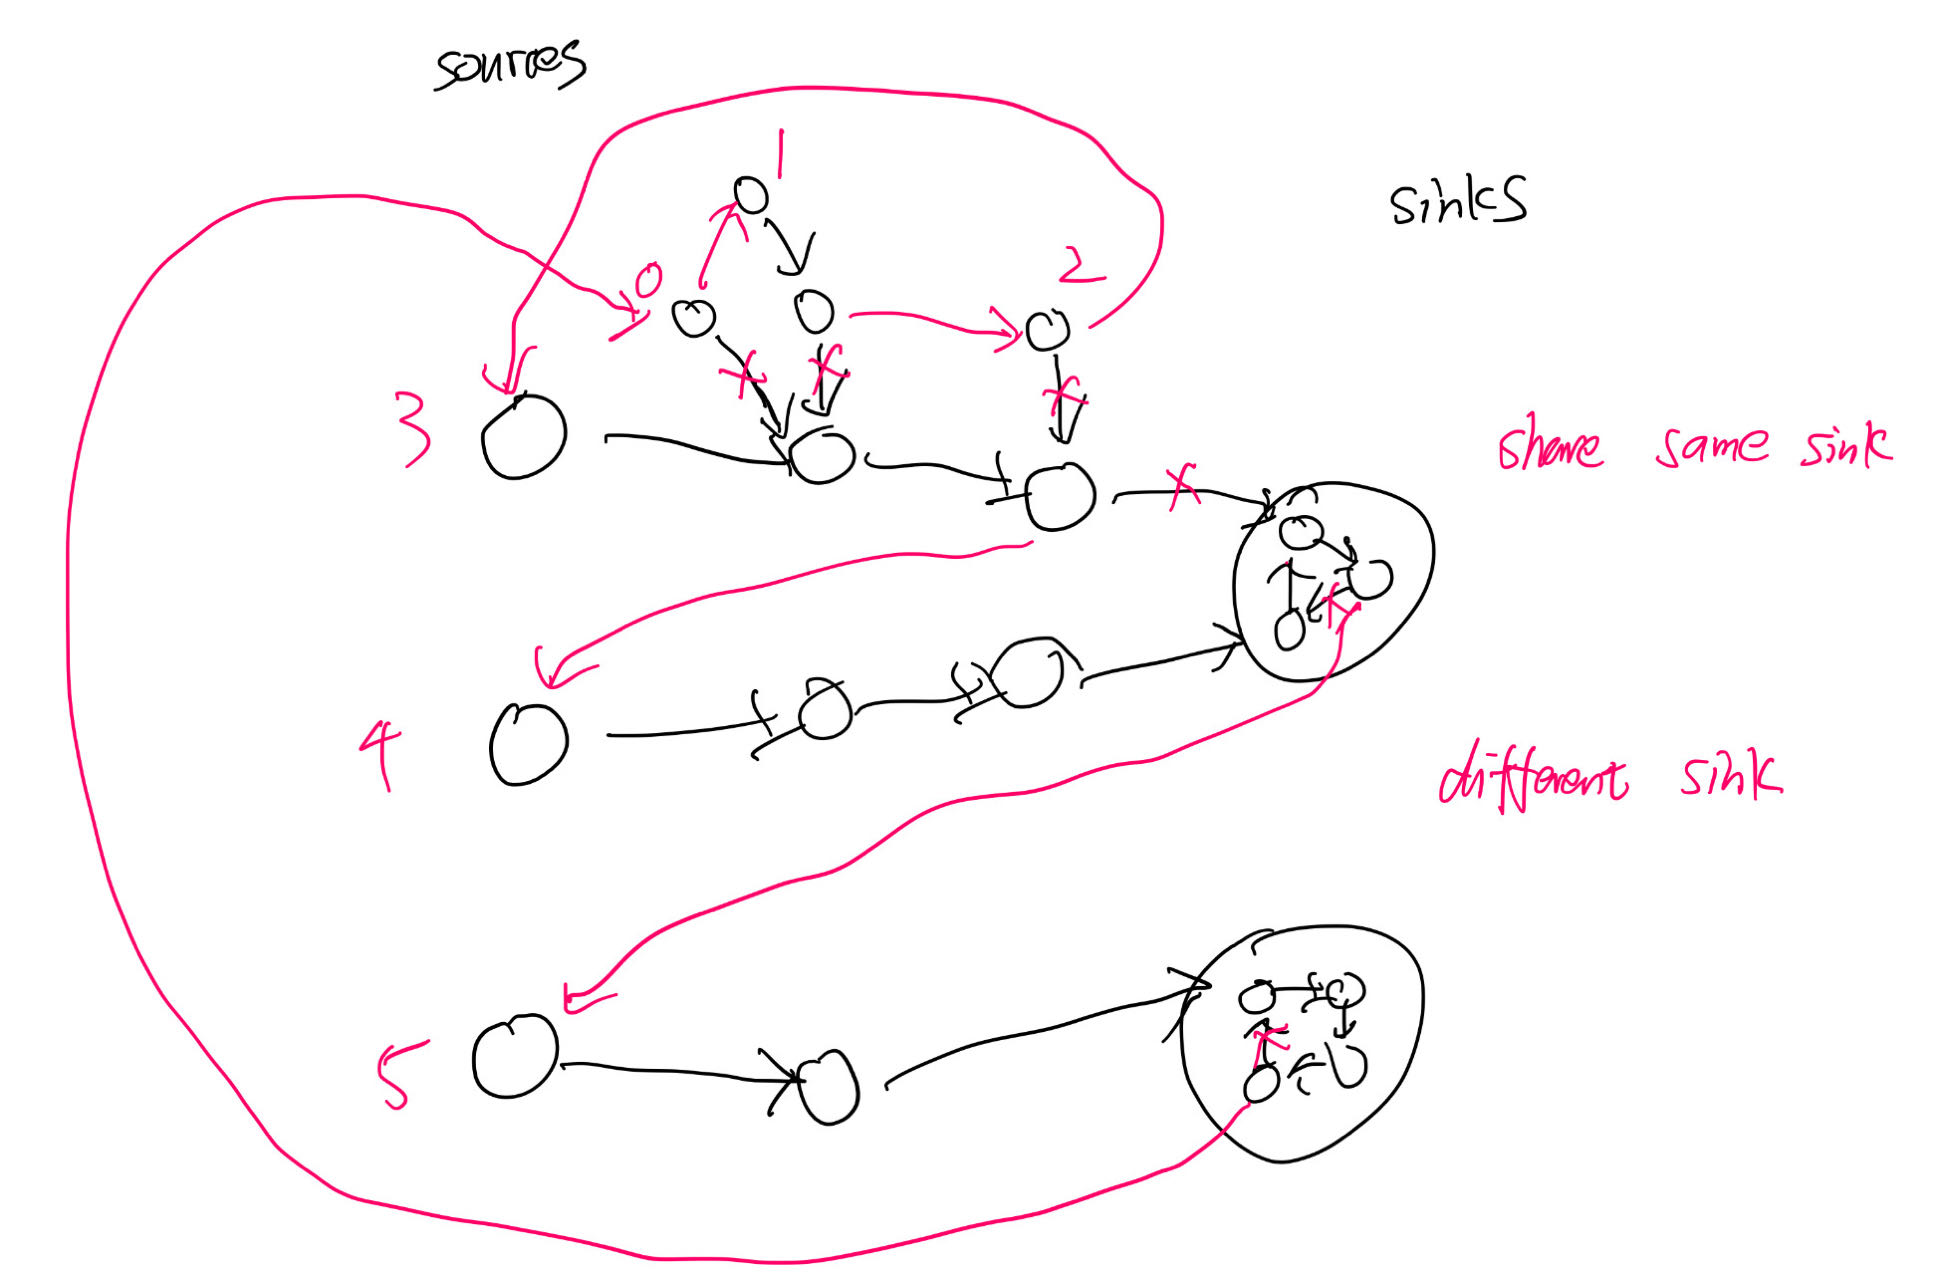
\includegraphics[width = 1\textwidth]{img/q24D.jpg}
\end{figure}

\newpage
Note that the algorithm records both the in-edge and out-edge of each vertex. Getting $G^{SCC}$ takes $O(n + n)$ time and iterating through sources takes approximately $O(2n)$ time in total. So the time complexity is $O(n)$

If sink $i$ has $k_i$ number of corresponding sources, we need to connect these sources together so that these sources are connected with each other. The reassignment number is $k_i - 1$.
Verticex in sink can't propagate to other vertices, but by connect one sink to another source, vertices can propagate to other vertices. All sinks need to be reassigned, so the reassignment number is number of sinks $|sinks|$. So the total number of reassignment is $|sinks| + \sum_{i = 0}^{|sinks|}(k_i - 1)$ or simply number of sources in $G^{SCC}$: $|sources|$

Through the above argument, it's clear that the algorithm builds a cycle containing all vertices. As has been approved, SCC sources in $G^{SCC}$ contains only one vertex so they are just vertices with in degree 0 in $G$. To enable any vertex to propagate to all vertices, at least these vertices need to be contacted. So in theory the minial number of reassignment is $|sources|$. The algorithm given achieves this.



\end{document}